\chapter{On Formal Languages} \label{chapter:2}
Formal languages are a fundamental concept in computer science, as they allow us to rigorously define and analyze the structure of different types of languages that we may encounter in both natural and artificial systems. 

Mateescu and Salomaa~\cite{handbook-formal-languages} explain a language as three possible explanations: 

\begin{enumerate}
    \item A body of words and systems for their use common to people of the same community or nation, geographical area, or cultural tradition
    \item A set or system of signs or symbols used in a more or less uniform fashion by a number of people that enables them to communicate and understand each other.
    \item Any system of formalized symbols, signs, gestures, etc. used as a means of communicating thought, emotion, etc.
\end{enumerate}

However, these provide a notion of ``language'' that is general rather than formal. When speaking of formal languages, it is essential to construct a systematic definition, or \emph{grammar}, rather than to consider a language as something given to us by others. 

To these effects, we will consider Hopcroft, Motwani and Ullman's~\cite{hopcroft-automata} definition of a language $\mathcal{L}$, as a set of strings chosen from $\Sigma^*$, where $\Sigma$ is a particular alphabet. An alphabet is defined as a finite, nonempty set of symbols. $\Sigma^*$ denotes the \emph{universal language}, which is the language formed by all possible sequences over an alphabet $\Sigma$.  For example, if we were to work with binary strings, $\Sigma = \{0, 1\}$ and $\Sigma^* = \{ \epsilon, 0, 1, 00, 01, 10, 11, 000, \cdots \}$. 

Formally, we define $\Sigma^*$ as the Kleene closure of $\Sigma$. The Kleene closure is defined, for a set of symbols $V \subseteq \Sigma$, as the set of all strings over symbols in $V$, including the empty string $\epsilon$, which can be expressed by the following equation~\cite{kleene-star}:

\begin{equation}\label{eq:kleene}
    V^* = \bigcup_{i=0}^{i=\infty} V^i
\end{equation}

Furthermore, they define a string or word as a finite sequence of symbols chosen from an alphabet $\Sigma$. Therefore, a word can also be seen as a concatenation of symbols that start with the \emph{empty} or \emph{identity} symbol, $\epsilon$.

However, not every word formed by the alphabet necessarily belongs to a language, since for each language, a specific set of rules exist that define \emph{membership} - whether a word belongs to the language or not. 

Once again, let us consider binary strings, but now we will restrict our language to those strings of even length. In this case, $\Sigma = \{ 0, 1\}$ and some valid strings in $\mathcal{L}$ would be $\{ \epsilon, 00, 11, 0011, \cdots \}$, but $\{ 0, 1, 010, 110, \cdots \}$ do not belong to $\mathcal{L}$ as they are not of even length.

Furthermore, it is important to note the existence of the \emph{empty language}, $\varnothing$, that is, the language that does not contain any words, not even the empty one - $\epsilon \notin \varnothing$. This is important, as it gives us a way to represent when a certain language cannot be constructed.

Even though the set of strings in a language may be infinite, these all stem from concatenations of a finite set, $\Sigma$, our alphabet. From this we can define a single constraint on what constitutes a language: its alphabet, $\Sigma$, must be a finite set~\cite{hopcroft-automata}.

\section{Chomsky's Hierarchy}
A grammar, according to Chomsky, is a set of rules or device that defines and enumerates the sentences of a languages. Also, these enumerators propose a set of restrictions, which then map to different types of automata, in such a way that  languagse that can be generated by a certain type of grammar are a proper subset of the less restrictive grammars~\cite{chomsky-hierarchy}.

For this work, we will focus on Type-2, or context-free grammars, which can be recognized by pushdown automata.The particularity of these grammars is they have a recursive, hierarchical structure and notation~\cite{hopcroft-automata}. For example, palindromes are a context-free language, as the grammar that generates it is also context-free.

\begin{figure}[h]
    \centering
    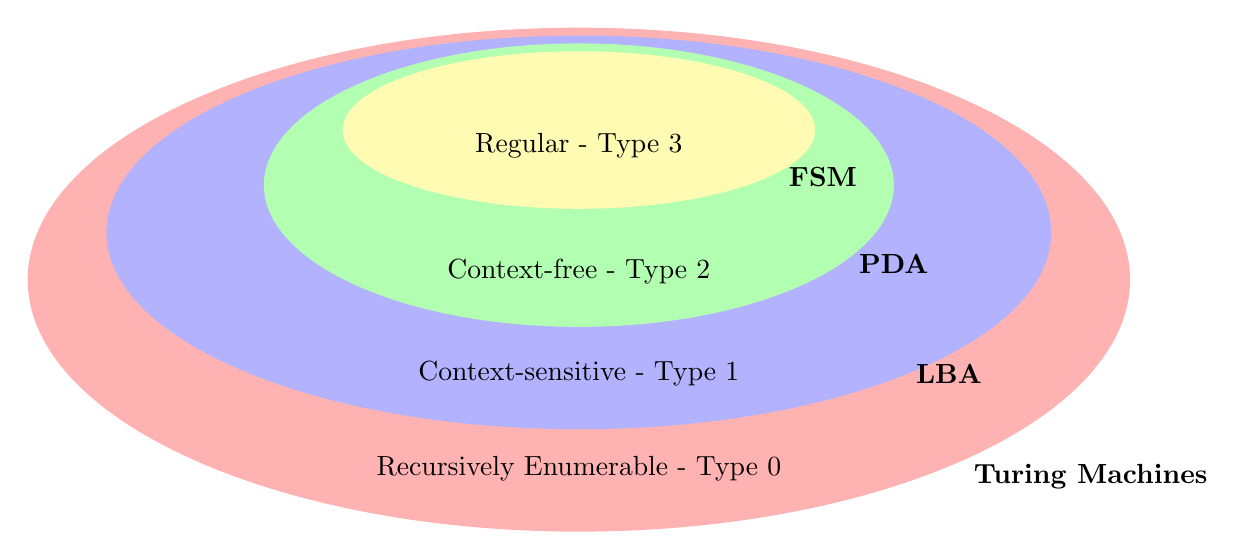
\begin{tikzpicture}
        % Draw ellipses for each language class
        \fill[red!30] (0, -0.2) ellipse (7 and 3.2);
        \fill[blue!30] (0, 0.4) ellipse (6 and 2.5);
        \fill[green!30] (0, 1) ellipse (4 and 1.8);
        \fill[yellow!30] (0, 1.7) ellipse (3 and 1);
    
        % Add labels inside each ellipse
        \node at (0, -2.6) {Recursively Enumerable - Type 0};
        \node at (0, -1.4) {Context-sensitive - Type 1};
        \node at (0, -0.1) {Context-free - Type 2};
        \node at (0, 1.5) {Regular - Type 3};

        \node at (3.1, 1.1) {\textbf{FSM}};
        \node at (4, 0) {\textbf{PDA}};
        \node at (4.7, -1.4) {\textbf{LBA}};
        \node at (6.5, -2.7) {\textbf{Turing Machines}};
    
    \end{tikzpicture}
    \caption{Chomsky Hierarchy}
    \label{fig:chomsky-fig}
\end{figure}

\subsection{Automata and Grammar Recognition}

From Chomsky's hierarchy, we gain insights into which type of automaton is expressive enough to recognize a particular type of language, as each type of grammar maps to a class of automaton. As we move from less restrictive languages to more restrictive languages, as seen in Figure~\ref{fig:chomsky-fig}, the automaton required to recognize the language becomes simpler.

\begin{itemize}
    \item Turing Machines: recognize any language.
    \item Linear-Bounded Automata (LBA): recognize context-sensitive languages.
    \item Pushdown Automata (PDA): recognize context-free languages. As these automata use a stack to keep track of symbols, they are particularly useful to recognize recursive laguages.
    \item Finite State Machines: recognize regular languages and are the simplest automata.
\end{itemize}

\section{Context-free grammars}
This work will focus on extracting attention patterns from Transformers trained on Type-2 grammars (context-free). We find these grammars of interest as they are central to the parsing of many modern programming languages and formal systems. Since they can represent recursive structures, they are particularly useful for defining constructs such as expressions, loops and function calls.

A context free grammar $\mathcal{G}$ has four main components~\cite{handbook-cfg, leeuwen-cfg}:
\begin{enumerate}
    \item A finite set of \emph{variables} $\mathbf{V}$ - these variables represent a language (a set of strings). We note $\mathbf{V}^*$ as the Kleene closure of the set of variables, as defined in Equation~\ref{eq:kleene}.
    \item A finite set of symbols $\mathbf{T}$, called \emph{terminals}. Note that $\mathbf{T} \subset \mathbf{V}$. Once again, $\mathbf{T}^*$ is the Kleene closure of the set.
    \item A \emph{start symbol} $\mathbf{S} \in \mathbf{V}-\mathbf{T}$.
    \item A finite set of \emph{productions}, $\mathbf{P} \subset (\mathbf{V}-\mathbf{T})\times \mathbf{V}^*$. These represent the recursive definition of the language. Each production consists of the following:
    \begin{enumerate}
        \item A variable, called the \emph{head} that is partially defined by the production.
        \item A production symbol $\rightarrow$
        \item A string of zero or more terminals and variables, called the \emph{body}.
    \end{enumerate}
\end{enumerate}

Therefore, a grammar $\mathcal{G}$ can be expressed as a four-tuple $(\mathbf{V}, \mathbf{T}, \mathbf{P}, \mathbf{S})$. 

Given 2 words, $u, v \in \mathbf{V}^*$, we say that $u \rightarrow v$ if there exists a derivation, or sequence of words in $\mathbf{V}^*$ such that $u_{i-1} \rightarrow u_{i}$ for $i = 1,\dots,k$ and $u_0=u$ and $v=u_k$. The existence of a derivation is noted by $u \xrightarrow{*} v$

Usually, grammars are presented with a notable nonterminal symbol, also called \emph{axiom}, noted by $\mathbf{S}$~\cite{hopcroft-automata, handbook-cfg}. The language generated by this variable in the grammar is called the \emph{language $\mathcal{L}$ generated by $\mathcal{G}$}  and can be defined as the following set:

\begin{equation}\label{eq:axiom-grammar}
\mathcal{L}(\mathcal{G}) = \{w \in \mathbf{T}^* | \mathbf{S} \xrightarrow{*} w \}
\end{equation}

Should $X$ be a variable in $\mathcal{G}$, then:

\begin{equation}\label{eq:variable-grammar}
\mathcal{L}_{\mathcal{G}}(X) = \{ w \in \mathbf{T}^* | X \xrightarrow{*} w\}
\end{equation}

From Equations~\ref{eq:axiom-grammar} and~\ref{eq:variable-grammar}, we derive that $\mathcal{L}(\mathcal{G}) = \mathcal{L}_{\mathcal{G}}(S)$. If two grammars generate the same language, they are considered \emph{equivalent}~\cite{leeuwen-cfg}.

\section{Dyck-$k$ Languages} \label{section:dyck_k}
Dyck-$k$ languages are a canonical family of context-free languages, composed of strings of balanced parentheses.
Let $A = \{ a_1, \dots, a_k \}$ and $\bar{A} = \{ \bar{a}_1, \dots, \bar{a}_k \}$. 
A Dyck-$k$ language is defined as a set of strings over the alphabet $\Sigma = A \cup \bar{A}$, where each string is a sequence of $2k$ parentheses, such that the parentheses are balanced. 
That is, for each string $w \in \Sigma^*$, the number of opening parentheses is equal to the number of closing parentheses, and for each prefix $w'$ of $w$, the number of opening parentheses is greater than or equal to the number of closing parentheses.

The language of Dyck-$k$ is denoted by $D_k$ and is defined by the following grammar:
\begin{align*}
    \mathbf{V} &= \{S\} \\
    \mathbf{T} &= \{a_1, \dots a_n\} \cup \{ \bar{a_1}, \dots, \bar{a_n} \}\\
    \mathbf{P} &= \{ S \rightarrow a_i S \bar{a_i} S | \epsilon \} \text{ for } i = 1, \dots, n \\
    \mathbf{S} &= \epsilon
\end{align*}

In this case, $\mathbf{T}$ is called a \emph{matched alphabet}, as each symbol $a_i$ has a corresponding closing symbol $\bar{a_i}$.

We say that Dyck-$k$ languages are canonical because they are the simplest form of context-free languages and can be used as a building block 
for all other context-free languages. This is known as the Chomsky-Sch{\"u}tzenberger Theorem \cite{rozenberg1997handbook} and states that a language $\mathcal{L}$ over an alphabet $\Sigma$ is context-free iff there exists:
\begin{itemize}
    \item a matched alphabet $A \cup \bar{A}$,
    \item a regular language $\mathcal{R}$ over $T \cup T'$,
    \item a homomorphism $h: {(T \cup T')}^* \rightarrow \Sigma^*$
\end{itemize}

such that $\mathcal{L} = h(R \cap D_T)$, where $D_T$ is the Dyck language over $T$.

It is useful to visualize a matched alphabet  $T \cup T'$ as matched parentheses, with $T$ being the set of opening parentheses and $T'$ the set of closing ones.

We find Dyck-$k$ languages interesting to study as they can showcase subject-verb agreement in common language (english, spanish, etc.)~\cite{bounded-hierarchical-languages}, therefore we can consider Dyck-$k$ languages as a sort of building block for common language. Furthermore, they are the canonical form of nested structures~\cite{context-free-chomsky}. We can see an example in the figure below:

\begin{figure}[h]
    \centering
    
    \tikzset{every picture/.style={line width=0.75pt}} 
    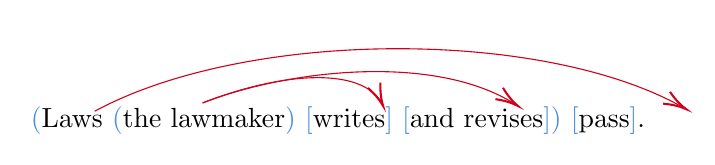
\begin{tikzpicture}[x=0.75pt,y=0.75pt,yscale=-1,xscale=1]
        \draw [color={rgb, 255:red, 208; green, 2; blue, 27 }  ,draw opacity=1 ]   (211,69.5) .. controls (284.63,29.7) and (427.56,29.5) .. (494.99,67.92) ;
        \draw [shift={(496,68.5)}, rotate = 210.2] [color={rgb, 255:red, 208; green, 2; blue, 27 }  ,draw opacity=1 ][line width=0.75]    (10.93,-3.29) .. controls (6.95,-1.4) and (3.31,-0.3) .. (0,0) .. controls (3.31,0.3) and (6.95,1.4) .. (10.93,3.29)   ;
        %Curve Lines [id:da30419908858250166] 
        \draw [color={rgb, 255:red, 208; green, 2; blue, 27 }  ,draw opacity=1 ]   (263,65.5) .. controls (302.77,49.98) and (339.72,48.57) .. (349.2,65.39) ;
        \draw [shift={(350,67)}, rotate = 246.61] [color={rgb, 255:red, 208; green, 2; blue, 27 }  ,draw opacity=1 ][line width=0.75]    (10.93,-3.29) .. controls (6.95,-1.4) and (3.31,-0.3) .. (0,0) .. controls (3.31,0.3) and (6.95,1.4) .. (10.93,3.29)   ;
        %Curve Lines [id:da5215279504274137] 
        \draw [color={rgb, 255:red, 208; green, 2; blue, 27 }  ,draw opacity=1 ]   (263,65.5) .. controls (303.59,49.66) and (374.56,41.17) .. (413.82,66.23) ;
        \draw [shift={(415,67)}, rotate = 213.69] [color={rgb, 255:red, 208; green, 2; blue, 27 }  ,draw opacity=1 ][line width=0.75]    (10.93,-3.29) .. controls (6.95,-1.4) and (3.31,-0.3) .. (0,0) .. controls (3.31,0.3) and (6.95,1.4) .. (10.93,3.29)   ;
        
        % Text Node
        \draw (179,66) node [anchor=north west][inner sep=0.75pt]   [align=left] {\textcolor[rgb]{0.29,0.56,0.89}{(}Laws \textcolor[rgb]{0.29,0.56,0.89}{(}the lawmaker\textcolor[rgb]{0.29,0.56,0.89}{)} \textcolor[rgb]{0.29,0.56,0.89}{[}writes\textcolor[rgb]{0.29,0.56,0.89}{] [}and revises\textcolor[rgb]{0.29,0.56,0.89}{]) [}pass\textcolor[rgb]{0.29,0.56,0.89}{]}.};
    
    \end{tikzpicture}
    \caption{Subject-verb agreement \cite{bounded-hierarchical-languages}}
    \label{fig:subject-verb-agreement}
\end{figure}

We see that this subject-verb agreement can be expressed by the Dyck-2 word \textcolor[rgb]{0.29,0.56,0.89}{( ( ) [ ] [ ] ) [ ]}.

Furthermore, Dyck-$k$ languages provide a way to easily parse and validate modern programming languages, for example, if we consider a C-like language, the expression shown in the figure below can be parsed by a Dyck-3 language:

\begin{figure}[h]
    \centering
    \begin{verbatim}
        foo( bar( arr[ index ] ), { key: value }, x + y )
    \end{verbatim}
    \caption{C-like expression}
    \label{fig:c-like-code}
\end{figure}

\paragraph{Shuffle-Dyck-$k$} \label{par:shuffle-dyck-k}

A particular, less restrictive case of Dyck-$k$ languages is given by the so-called Shuffle-Dyck-$k$ family of languages.

This family of languages is made up of $k$ shuffles of Dyck-1 languages, with $k$ different types of brackets. Each type of bracket must be well balanced, but there is no restriction to their relative order~\cite{bhattamistra-transformers-formal-languages}.